%%%%%%%%%%%%%%%%%%%%%%%%% CHAPTER 1%%%%%%%%%%%%%%%%%%%%%%%%%%%%%%%%

\chapter{Experimentos y Resultados} \label{experimentos}
% Descripción del problema
\section{Descripción del problema}
Para la fase experimental se utilizaron dos bases de datos. Como punto comparativo al actual estado del arte, se utilizó 
% el CIFAR10 \cite{CIFAR}. Además, se hizo uso de 
una base de datos provista por el \textsl{Pollen Challenge} \cite{polen}. El objetivo del concurso era clasificar los granos de polen utilizando un  conjunto de imágenes bajo microscopio.

Las imágenes de microscopio fueron digitalizadas y clasificadas por expertos aerobiológicos en 4 clases, las cuales incluyen 3 especies de polen y una clase extra que podría ser confundida con polen (burbujas, aire, etc). 
\begin{figure}[H]
    \centering
    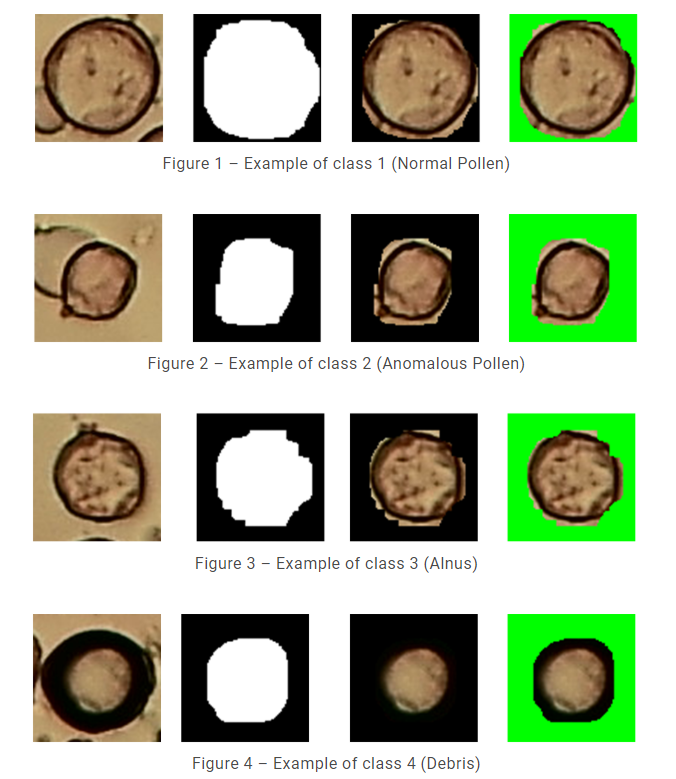
\includegraphics[width = 5in]{../cap5_experimentos/src/polen.png}
    \caption{Imagen extraída de la página oficial del Pollen Challenge \cite{polen}}
\end{figure}
% Métricas
\section{Métricas para clasificación Binaria}
% Accuracy
Analizaremos primero el caso de las métricas en un problema de clasificación binario. Es decir, dada una clase $\mathcal C$, es posible que un dato $y$ pertenezca o no pertenezca a $\mathcal{C}$.

Es importante describir primero las métricas en este tipo de problemas, debido a que cuando nos adentremos a la clasificación multiclase, estas métricas nos serán de utilidad.
\subsection{Matriz de confusión}
Considérese un problema de clasificación binario. En el mejor de los casos, el modelo podría predecir perfectamente qué datos pertenecen a la clase y cuáles no lo hacen. Sin embargo, siendo que es un modelo estadístico, el modelo no siempre acertará, y usando los datos etiquetados se puede detectar en dónde ha habido una \textsl{confusión}. El modelo puede confundirse de dos maneras: La primera es afirmando que $y\in \mathcal C$ cuando no es el caso, y la segunda es clasificar  $y\notin \mathcal C$, cuando en realidad $y$ sí pertenecía a la clase. Por tanto, existen 4 posibilidades:

\begin{enumerate}
    \item \textbf{Verdaderos positivos}: Aquellos datos que sí pertenecen a la clase, y fueron clasificados dentro de la clase. A la cantidad de verdaderos positivos se le denota $T_P$ por sus siglas en inglés.
    \item \textbf{Falsos positivos}: Aquellos datos que sí pertenecen a la clase, y fueron clasificados fuera de la clase. A la cantidad de falsos positivos se le denota $F_P$ por sus siglas en inglés.
    \item \textbf{Verdaderos negativos}: Aquellos datos que no pertenecen a la clase, y fueron clasificados fuera de la clase. A la cantidad de verdaderos negativos se le denota $T_N$ por sus siglas en inglés.
    \item \textbf{Falsos negativos}: Aquellos datos que no pertenecen a la clase, y fueron clasificados dentro de la clase. A la cantidad de falsos negativos se le denota $F_N$ por sus siglas en inglés.
\end{enumerate}
Es posible agrupar toda esta información en una matriz conocida como \textsl{matriz de confusión}. 
\begin{definition}
    \label{pos_neg}
    Considérese el problema de clasificación (\ref{clasification}) con $m = 2$. Sea $f: \mathbb R^n \to C$ el modelo. Definimos los siguientes valores:
    \begin{align*}
        T_P = |\{y_i : c_i &= (1,0)^T \text{ y } f(y_i) = (1,0)^T\}| \\
        F_P = |\{y_i : c_i &= (0,1)^T \text{ y } f(y_i) = (1,0)^T\}| \\
        T_N = |\{y_i : c_i &= (0,1)^T \text{ y } f(y_i) = (0,1)^T\}| \\
        F_N = |\{y_i : c_i &= (1,0)^T \text{ y } f(y_i) = (0,1)^T\}|.
    \end{align*} 
    La matriz de confusión se define como 
    \begin{equation}
        D = \left[\begin{matrix}
            T_P & F_P \\
            F_N & T_N
        \end{matrix}\right].
    \end{equation}
\end{definition}
\begin{figure}[H]
    \centering
    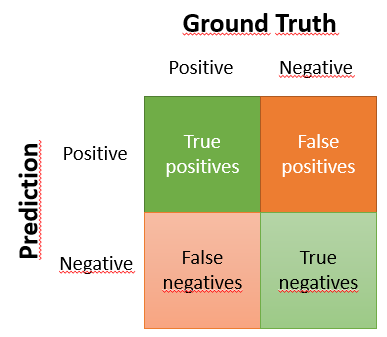
\includegraphics{../cap5_experimentos/src/matriz_confusion_binaria.png}
    \caption{\textcolor{red}{Conseguir imagen propia}}
\end{figure}
%------------- Accuracy
\subsection{Exactitud}
La exactitud se define como la razón de las predicciones acertadas y las predicciones totales. En el aprendizaje automático suele ser la métrica principal, ya que determina el porcentaje de aciertos. Sin embargo, no es el único factor  a tomar en cuenta.
\begin{definition}[exactitud]
    Considérese los valores $T_P, F_P, T_N, F_N$ de la definición (\ref{pos_neg}). La exactitud $A$ se define como 
    \begin{equation}
        A = \frac{T_P + T_N}{T_P + F_P + T_N + F_N}
    \end{equation}
\end{definition}
%------------- Sensibilidad y Especificidad
\subsection{Sensibilidad y Especificidad}
Existen ocasiones en las que no es conveniente utilizar la Exactitud como único criterio del desempeño, especialemente cuando se tiene un conjunto de datos desbalanceado (Sección \ref{unbalanced_sets}). Por ejemplo, al detectar llamadas fraudulentas, no servirá usar la Exactitud, porque casi ninguna llamada es fraudulenta. Lo conveniente sería conocer cuántas veces se acertó al tratar de predecir resultados negativos (Especificidad) o viceversa, cuántas veces se acertó al tratar de predecir resultados positivos (Sensibilidad). 

\begin{definition}
    Considérese los valores $T_P, F_P, T_N, F_N$ de la definición (\ref{pos_neg}). La sensibilidad $R$ y la especificidad $E$ se definen respectivamente como 
    \begin{equation}
        R = \frac{T_P}{T_P + F_P}
    \end{equation}
    \begin{equation}
        E = \frac{T_F}{T_F + F_N}
    \end{equation}
\end{definition}
%------------- Precisión
\subsection{Precisión}
\begin{definition}[Precisión]
    Considérese los valores $T_P, F_P, T_N, F_N$ de la definición (\ref{pos_neg}). La precisión $P$ se define como 
    \begin{equation}
        P = \frac{T_P}{T_P + F_P}
    \end{equation}
\end{definition}
%------------- F1-score
\subsection{\textcolor{red}{F1-score}}
En algunos problemas, es necesario tomar en cuenta la precisión y la sensibilidad por igual. La F1-score, propuesta en 2006 en \cite{f1score}, se define como la media armónica de estas dos métricas. 
\begin{definition}[\textcolor{red}{F1-score}]
    Considérese los valores $T_P, F_P, T_N, F_N$ de la definición (\ref{pos_neg}). La \textcolor{red}{F1-score} $F_1$ se define como 
    \begin{equation}
        F_1  = \frac{2}{\frac{1}{R} + \frac{1}{P}} = \frac{2RP}{R + P} = \frac{T_P}{T_P + \frac{1}{2}(F_P + F_N)}
    \end{equation}
\end{definition}
\begin{figure}[H]
    \centering
    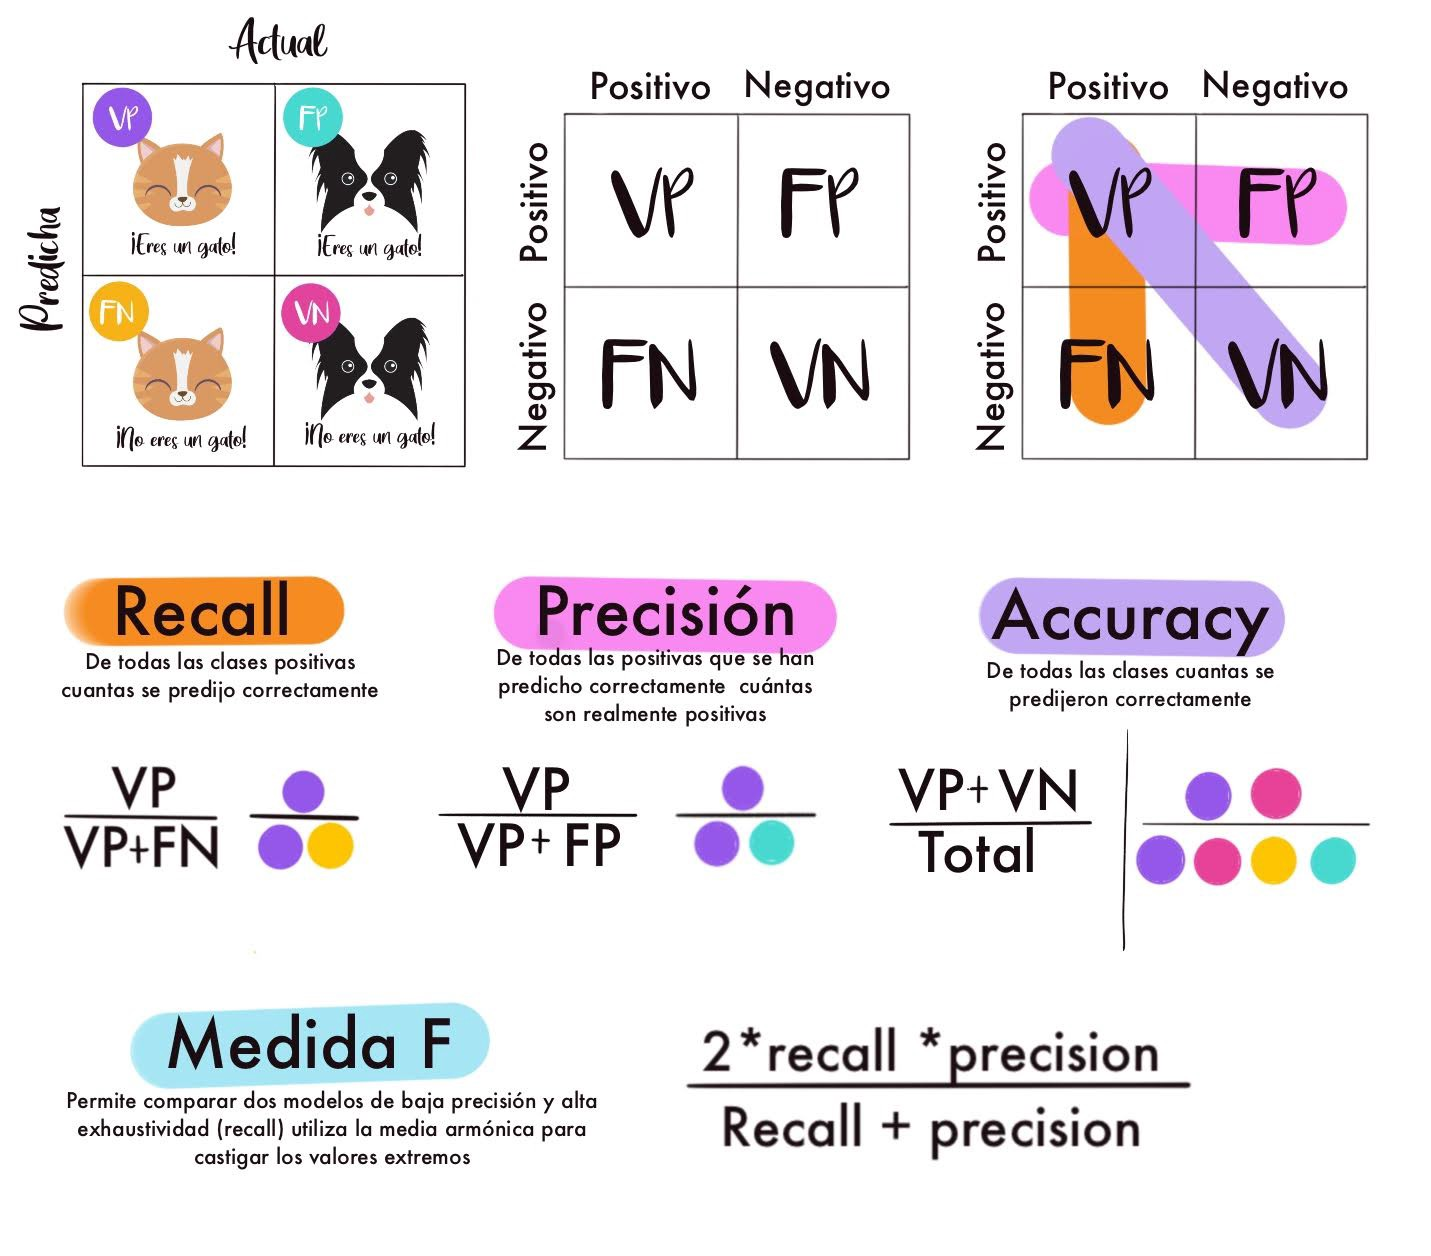
\includegraphics[width=4in]{../cap5_experimentos/src/metricas.jpeg}
\end{figure}
\section{Métricas para clasificación multiclase}
En cuanto a la problema de clasificación con $m$ clases, no podemos hacer uso directo de las todas las fórmulas anteriores. Sin embargo, es posible conseguir una matriz de confusión. En este caso, el eje $x$ determina la verdadera etiqueta, y el eje $y$ determina la etiqueta predicha por el modelo.

De modo que la matriz de confusión para el problema de clasificación multiclase es de la siguiente forma:
\begin{equation}
    D = \left(\begin{matrix}
        d_{1,1} & d_{1,2} & \cdots & d_{1,m} \\
        d_{2,1} & d_{2,2} & \cdots & d_{2,m} \\
        \vdots & \vdots & \ddots & \vdots \\
        d_{m,1} & d_{m,2} & \cdots & d_{m,m} 
    \end{matrix}\right),
\end{equation}
dónde $d_{i,j}$ es la cantidad de elementos pertenecientes a la clase $j$ que fueron clasificados en la clase $i$. Por tanto, un modelo que clasifique todas las instancias correctamente, tendrá una matriz de confusión diagonal.  

\begin{definition}
    Sea $D$ una matriz de confusión, su versión normalizada se determina por la regla 
    \begin{equation}
        \hat d_{i,j} = \frac{d_{i,j}}{|C_i|}
    \end{equation}
\end{definition}

Es sencillo definir la forma generalizada de la Exactitud, basándonos en que es la razón entre la cantidad total de aciertos (La suma de los elementos en la diagonal de la matriz de confusión) y la cantidad total de instancias, es decir la suma de cada entrada de la matriz.
\begin{definition}
    Sea $D$ una matriz de confusión. Se define la exactitud $A$ de la siguiente manera:
    \begin{enumerate}
        \item Exactitud:
        \begin{equation}
            A = \frac{\sum_{i=1}^n d_{i,i}}{\sum_{i,j} d_{i,j}}
        \end{equation} 
    \end{enumerate}
\end{definition}
\begin{figure}[H]
    \centering
    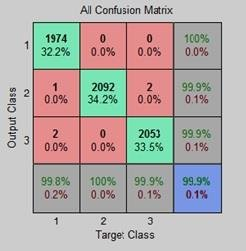
\includegraphics{../cap5_experimentos/src/confision_multiclase.png}
    \caption{\textcolor{red}{Conseguir imagen propia}}
\end{figure}

Por otro lado, para las métricas de Precisión y Sensibilidad se tienen dos posibles definiciones: La \textsl{Macro} y la \textsl{Ponderada}.


 %------------- Macro
 \subsection{Métricas Macro}

 %------------- Ponderada
 \subsection{Métricas Ponderadas}
